This section covers the essential concepts related to Concurrent Stochastic Multi-player Games and their implementation in PRISM games. \cmt{Furthermore, We will revisit the AMQP protocol stack, which is essential for understanding message routing.}

\subsection{Concurrent Stochastic  Games}
Concurrent stochastic games (CSGs) \cite{kwiatkowskaautomatic2021, fismancorrelated2022} consider that players make choices concurrently in each state and then transition simultaneously. In CSGs, players have control over one or more modules, and the actions associated with these modules can only be utilized by the respective player who owns them. The CSG is defined as an extension of Probabilistic Automata (PA) \cite{ref27} in \cite{kwiatkowskaautomatic2021, fismancorrelated2022} as follows:

%This makes CSGs distinct from approaches to automata synchronization based on common action labels. 

\begin{mydef} \label{def:csg} \normalfont A concurrent stochastic multi-player game (CSG) is a tuple \emath{G =\gl{s_{0}, S, N, A, \Delta, \delta, AP, L}}:

\begin{itemize}
	\item \emath{s_{0}} is an initial state, such that \emath{s_{0} \in S},
	\item \emath{S} is a set of states,
	\item \emath{N =\{1,...,n\}} is a finite set of players,
	 \item \emath{A= \Sigma_{1} \times \ldots \times \Sigma_{n} } where \emath{\Sigma_{i}} is a finite set of actions available to player \emath{i \in N},
     \item \emath{\Delta: S \longrightarrow 2^{\cup_{i=0}^{n} \Sigma_{i}}} is an action assignment function,
 
    \item \emath{\delta : S \times A \longrightarrow Dist(S)} is a probabilistic transition function assigning for each \emath{s \in S} and \emath{(\alpha_{0},\ldots, \alpha_{n}) \in \Sigma_{i} } a probabilistic distribution \emath{\mu \in Dist(S)}, and \emath{L: S \longrightarrow 2^{AP}} is a labeling function that assigns each state  \emath{s \in S}  to a set of atomic propositions taken from the set of atomic propositions (\emath{AP}).
\end{itemize}
\end{mydef}


When in state s, each player \emath{i \in N} selects an action from its available actions \emath{Action_{i}(s) \myeq \Delta(s) \cap \Sigma_{i}} if this set is non-empty.  A path \emath{\pi} of a CSG \emath{G} \cite{kwiatkowskaautomatic2021, fismancorrelated2022} is a sequence \emath{\pi = s_{0}\xrightarrow{\alpha_{i}}s_{1}} where \emath{s_{i} \in S}, \emath{\alpha_{i} = (a_{j}^{1}, . . . , a_{j}^{n}) \in A}, \emath{\alpha_{i}^{j} \in Action_{i} (s_{i})} for \emath{i \in N} and \emath{\delta(s_{j}, \alpha_{j})(s_{j+1}) > 0} for all \emath{j > 0}. 


CSGs are augmented with reward structures \cite{kwiatkowskaautomatic2021}  as \emath{r_{A} : S \times A \longrightarrow \mathbb{R}} is an action reward function that assigns a real value to each pair of state and action tuples, which accumulates when the action tuple is selected in the corresponding state and \emath{r_{s} : S \longrightarrow \mathbb{R}}  is a state reward function assigns a real value to each state, which accumulates when the state is reached.


The properties related to CSGs are expressed in the temporal logic rPATL \cite{hutchisonautomatic2012} (reward Probabilistic Alternating Temporal Logic). The property grammar is based on CTL \cite{baierprinciples2008} extended with coalition operator \emathtt{\langle\langle C\rangle\rangle} of ATL \cite{Alur2002} and probabilistic operator \emathtt{P} of PCTL \cite{hanssonlogic1994}. For instance, for the following property expressed in natural language: \quot{\emph{Players 1 and 2 have a strategy to ensure that the probability of shutdown occurring within 100 steps is less than 0.001, regardless of the strategies of other players}} is expressed in rPATL as: \emathtt{\langle\langle 1,2\rangle\rangle P_{<0.001} [ F^{\leq100} shutdown].} Here, \quot{\emathtt{shutdown}} is the label that refers to the system states. Concerning rewards structure, the property expressed in natural language: \quot{\emph{What is the maximum commutative reward r within 100 steps to reach \quot{\emathtt{fail}} for both Players 1 and 2 for a selected strategy ?}} is expressed  in rPATL as \emathtt{\langle\langle 1,2\rangle\rangle R _{max=?} [ C^{\leq 100}] }

\begin{example}
\label{exp:csg:architecture}   
Consider the CSG shown in \fig{fig:even:odds}, which corresponds to two players repeatedly performing a scheduled read and write operation. Transitions are labeled with actions where \emath{A = (r_{1}r_{2}), (w_{1}w_{2}), (w_{2}r_{1}), (r_{2}w_{2}), (reset_{1} reset_{2})}. The CSG starts in state 's0', and states 's1', 's2', and 's3' are labeled with atomic propositions corresponding to a player winning. Each player communicates through writing and reading operations.
%\tikzset{every picture/.style={ scale=0.95,line width=0.2pt}} %set default line width to     
\noindent
\begin{figure}[!htb]
    \centering
  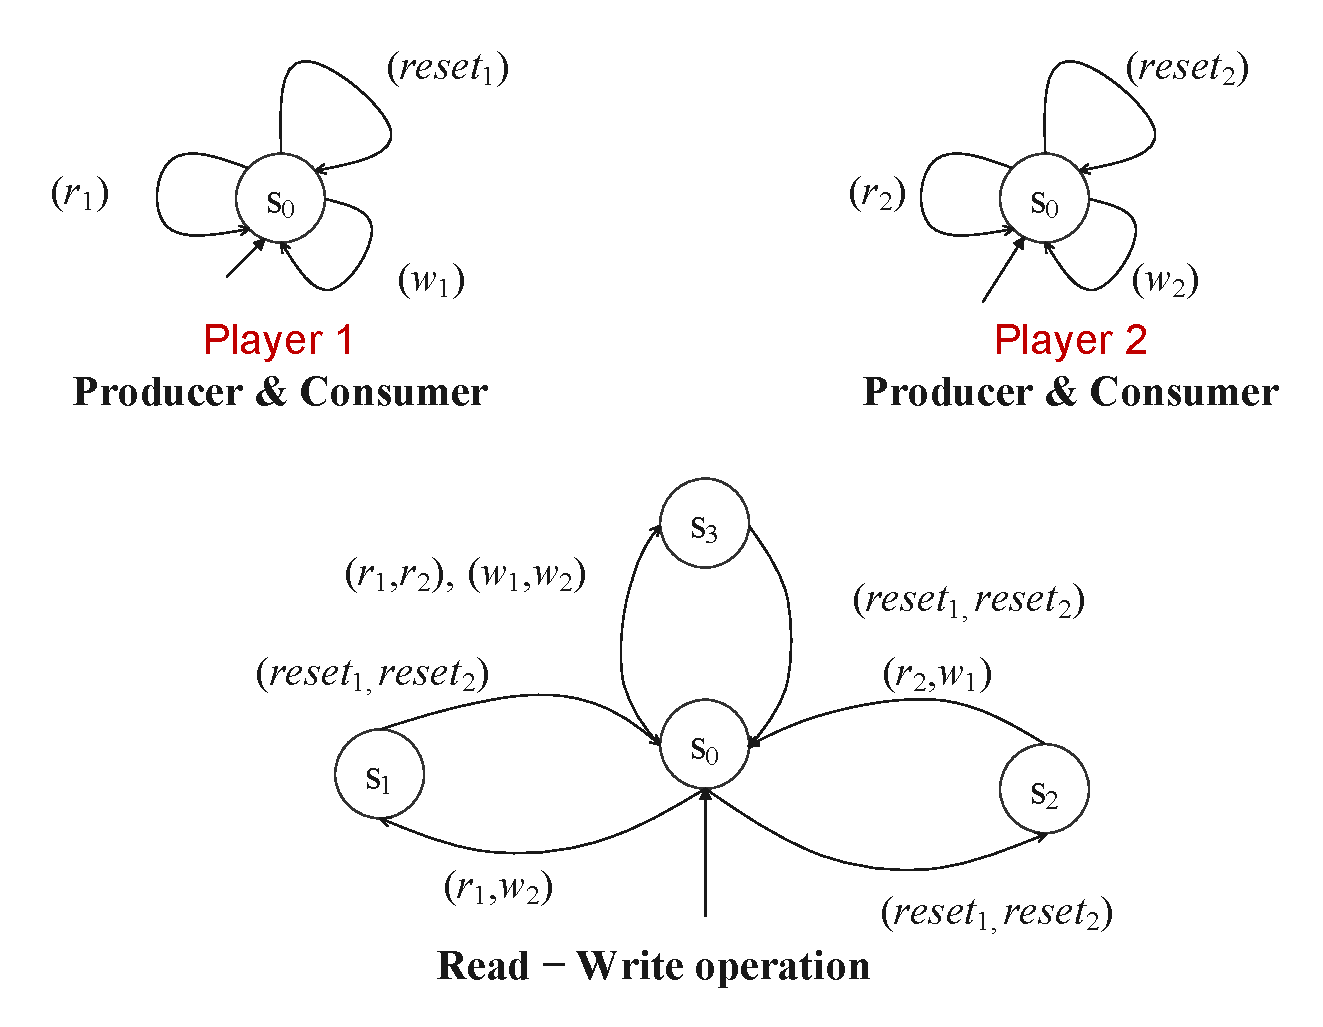
\includegraphics[width=250pt, height =200pt]{examplecsg.pdf}
    \caption{Read and Write Game Model in CSG.}
    \label{fig:even:odds}
\end{figure} 

In relation to the modeled system, if Player 1 commences the game and that player emerges victorious as it performs writing, the property is expressed as \emathtt{\langle\langle 1,2 \rangle\rangle P_{>0.99}=? [ F \ win=1 ]}. The model and properties associated with the example are available at \cite{edcc23}. 

\end{example}
%\end{paperexample}

\subsection{The PRISM-games language}
We rely on the CSG model to express the coalition game in PRISM language \cite{Kwiatkowskaprism2011}. The PRISM model is composed of a set of modules that can synchronize. A set of variables and commands characterizes each module. The variable's valuations represent the state of the module. A set of commands is used to describe the behavior of each module (i.e., transitions). A command takes the form: \emath{ [a_{j}, \ldots, a_{m}] g \rightarrow \lambda_{1}: u_{1} + \ldots+ \lambda_{n}: u_{n} } or, \emath{[a_{j}, \ldots, a_{m}] g \rightarrow u}, which means, for actions \quot{\emath{a}} if the guard \quot{\emath{g}} is true, then, an update \quot{\emath{u_{i}}} is enabled with a probability \quot{\emath{\lambda_{i}}}. A guard is a logical proposition consisting of variable evaluation and propositional logic operators. The update \quot{\emath{u_{i}}} is an evaluation of variables expressed as a conjunction of assignments: \emath{v_{i}'=val_{i}+\ldots+v_{n}'=val_{n}} where \quot{\emath{v_{i}}} are local variables and \emath{val_{i}} are values evaluated via expressions denoted by \quot{\emath{eval}} such that \emath{ eval: V \rightarrow \mathbb{D}}.
Let \emath{\mathbb{D}} be a domain of variables such as \emath{\mathbb{D}=\mathbb{N} \cup \{true,false\} }. We define valuations for variables as \quot{\emath{\theta}} such that \emath{ \theta: V \rightarrow \mathbb{D} } that associate each variable in \emath{V} with a value in \emath{\mathbb{D}}. We use \emath{l_{0}, l_{1},\ldots, l_{n}} as new valuations of variables \emath{v_{0}, v_{1},\ldots, v_{n}}. Each PRISM command is encapsulated within a PRISM module \cite{KWIATKOWSKA20065} defined as follows:

\begin{mydef} \label{def:prismmodule} \normalfont (PRISM-Module). A PRISM module \quot{\emath{\mathcal{D}}} is a tuple \emath{\mathcal{D}= \langle \vartheta_{L}, Cm\rangle}, where: 
 \begin{itemize}
\item \emath{\vartheta_{L}} is a finite set of local variables associated with the module \emath{\mathcal{D}} initialized with \emath{init},
\item \emath{Cm} is a finite set of commands that defines the behavior of module \emath{\mathcal{D}}. Formally, we consider the command of the form \emath{ [a_{0}, \ldots, a_{m}] g \rightarrow \lambda: u} as \emath{l_{i}\xrightarrow{g:\gl{ a_{j}, \ldots, a_{m}}}_{\lambda}l'_{i}} such that \emath{l_{i}\models g}, \emath{g \in Const(V)} and \emath{\theta':=\theta[v_{i}:=eval(v_{i})]}.
            \end{itemize}
\end{mydef}

\begin{example}
In the PRISM code of \lst{exampleinprism}, a dedicated non-player module  is used for orchestrating read and write operations. All commands are labeled with at least two ports, which correspond to the players responsible for triggering the internal write and read operations. The "win" variable defines the player's success in writing (taking values 1 or 2).
The first commands shown in lines 5-6 represent unscheduled writing (i.e., reading) operations. As these operations are executed, a reset command is introduced in line 8 to indicate an idle state. Subsequently, the commands depicted in lines 9-10 enforce an order between writing and reading operations.  The model and properties associated with the example are available at \cite{edcc23}.

\lstdefinestyle{framed}
{
	frame=lrb,         
	mathescape,
	numbers=left,
	belowcaptionskip=-1pt,
    xleftmargin=3em,
		xrightmargin=0.01cm,
    framexleftmargin=3em,
	framexrightmargin=0pt,
	framextopmargin=5pt,
	framexbottommargin=5pt,
	framesep=0pt,
	rulesep=0pt,
	numbers=left,
}
    
\lstset{
    breaklines=true,
    style=framed,
    escapeinside={<@}{@>},
    morekeywords={void, int, public, private, class, protected, submodules, network, connections, const, init, int, bool, double, module, rewards, endrewards, endmodule},
    basicstyle=\ttfamily,
    keywordstyle=\bfseries\color{blue},
        morecomment=[f][\color{green!30!black}][0]{/*},
    morecomment=[l][\color{green!30!black}]{//},
    label=queueemodel
}



\begin{figure}[!htb]            
\begin{minipage}{15.5cm}
\begin{lstlisting}[style=framed,%customc,
	caption=PRISM Code for Read/Write of \fig{fig:even:odds},
 	label=exampleinprism]	
module recorder // a non player model in charge of recording players actions
 win : [0..2]init 0;
 a : [0..2]init 0;
	
 [w1,w2] s=0 -> (s'=1) & (win'=0);
 [r1,r2] s=0 -> (s'=1) & (win'=0);

 [reset1,reset2] s=1 | s=2 | s=3 -> (s'=0) & (win'=0);
 [r1,w2] s=0 -> (s'=2) & (win'=2);
 [w1,r2] s=0 -> (s'=3) & (win'=1);
endmodule
\end{lstlisting}
 \end{minipage}  
\end{figure}

\end{example}

\subsection{The RabbitMQ broker}
\cmt{RabbitMQ, a message broker, implements the Advanced Message Queuing Protocol (AMQP), standardized in ISO/IEC 19464:2014 \cite{ISOAMQP}. AMQP defines the communication rules for messages where RabbitMQ serves as a concrete implementation. This paper utilizes the AMQP 0.9/1.0 implementation provided by RabbitMQ \cite{Rabbitmq}. The reference communication stack, depicted in \fig{fig:rabbitmq:arch}, is adapted from the AMQP Architecture specification (AMQP Architecture:  \cite{Rabbitmq} and \cite{amqp-architecture}). (1) Application Layer: This layer interacts with applications using client libraries and defines a message format and semantics (\emph{see section 2.1 AMQ Model Architecture} in  \cite{Rabbitmq}). (2) Messaging Layer: This layer handles message routing, exchanges, queues, and bindings (\emph{see section 3.1.1 Messages and Content} in \cite{Rabbitmq}), with a focus on message routing and distribution. (3) Framing Layer: This layer takes messages from the messaging layer and packages them into frames with specific headers and content data (\emph{see section 2.3.5 Frame Details} in  \cite{Rabbitmq}), focusing on data structuring and encapsulation. (4) Transport Layer: This layer provides reliable and secure communication between peers (RabbitMQ clients/servers). It typically uses TLS/SSL for encryption and TCP for reliable delivery (\emph{many features are discussed in section 2.3 AMQP Transport Architecture} in  \cite{Rabbitmq}). (5) Wire Level: This layer defines the byte format on the network for each frame (\emph{see section 4.2 AMQP Wire-Level Format} in \cite{Rabbitmq}), addressing low-level network communication details.}

\noindent
\begin{figure}[!htb]
    \centering
  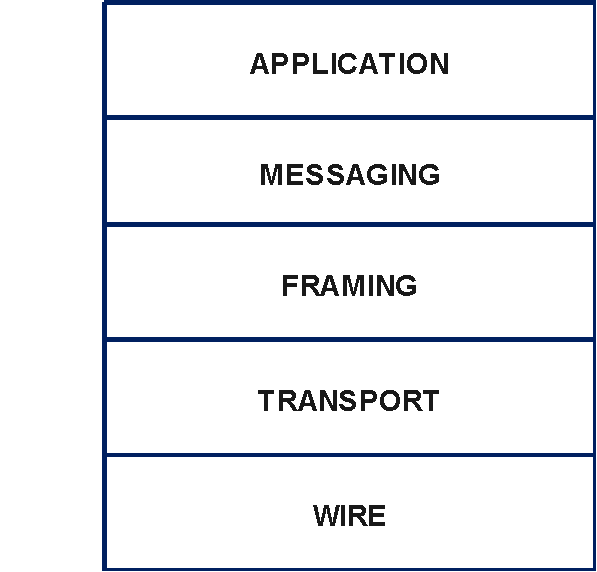
\includegraphics[width=170pt, height =190pt]{architecture.pdf}
    \caption{RabbitMQ Implementation of AMQP Architecture\cite{amqp-architecture}.}
    \label{fig:rabbitmq:arch}
\end{figure} 

The main feature that can justify the use of the RabbitMQ broker for IoT implementing AMQP and in the case of IoT gateway \cite{sensinactref2024, Baouyasaddek2024} is \cmt{the implementation of a CoAP-to-RabbitMQ. It can bridge the communication gap between resource-constrained devices and robust messaging systems. This bridge translates CoAP messages into the richer format used by RabbitMQ. This approach fosters interoperability, allowing diverse device types to participate in a unified communication ecosystem supported by gateways in \cite{sensinactref2024}. In addition, RabbitMQ broker implements clustering functions \cite{rabbitmq-clustering} that enhance the availability and reliability of the infrastructure.}


